\section{System Control}

\begin{frame}
\frametitle{RCM Tracking}

\begin{columns}
\column{0.5\textwidth}
\begin{center}
\begin{figure}[!htb]
\centering
\includegraphics[width=0.8\textwidth]{../images/robot_planner6/rcm-error-geometry.png}
\caption{Geometric calculation of the RCM alignment error $e$ using the distance between the line $l$ and the RCM point.}
\label{rcm-error-geometry}
\end{figure}
\end{center}

\column{0.5\textwidth}
\[
{}^UT_{T0} = \begin{bmatrix}
\mathbf{\hat{x}} & \mathbf{\hat{y}} & \mathbf{\hat{z}} & \mathbf{p} \\
0                & 0                & 0                & 1 \\
\end{bmatrix}
\]

\[
\overrightarrow{O_FA} = \mathbf{p}, \quad \textrm{and} \quad \overrightarrow{O_FB} = \mathbf{p} + \mathbf{\hat{x}}
\]

\[
e_{rcm} = d(l, O_F)
\]

\[
d(l, O_F) = \frac{\Vert \overrightarrow{O_FA} \times \mathbf{\hat{x}} \Vert}{\Vert \mathbf{\hat{x}} \Vert}
\]
\end{columns}
\end{frame}


\begin{frame}
\frametitle{RCM Tracking}
\begin{columns}
\column{0.5\textwidth}
\begin{center}
\begin{figure}[!htb]
\centering
\includegraphics[width=0.8\textwidth]{../images/rcm-force-interaction-model.png}
\caption{Force interaction model of the laparoscopic tool and the abdominal wall around the fulcrum point (RCM point)}
\label{rcm-force-interaction-model}
\end{figure}
\[
\Vert \mathbf{f}_s \Vert = \frac{λ}{cosγ} e 
\]
\end{center}


\column{0.5\textwidth}
\begin{center}
\begin{figure}[!htb]
\centering
\includegraphics[width=0.6\textwidth]{../images/rcm-error-yz.png}
\caption{RCM error calculation in yz plane. The RCM error or yz-error is the distance between the line of the $\mathbf{\hat{x}}$ vector (here seen as a point) and the estimated position of the origin of the
fulcrum reference frame $\tilde{O}_F$}
\label{rcm-error-yz-plane}
\end{figure}
\end{center}

\end{columns}
\end{frame}

\begin{frame}
\frametitle{RCM Tracking}
\begin{center}
\begin{figure}[!htb]
\centering
\includegraphics[width=\textwidth]{../images/rcm-system-control.png}
\caption{RCM tracking proposed control system. The RCM error is used as input in the trajectory generator to correct the trajectory command in order to fix the RCM misalignment}
\label{rcm-control-system-block-diagram}
\end{figure}
\end{center}
\end{frame}


\begin{frame}
\frametitle{Image based visual servoing}
\begin{center}
\begin{figure}[!htb]
\centering
\includegraphics[width=0.45\textwidth]{../images/visual_servo_start.png}
\includegraphics[width=0.45\textwidth]{../images/visual_servo_end.png}\\
\caption{Image based visual servoing. The robot arm is controlled using the information gained from the video frames. The frames are 2-Dimensional and thus 
the detected objects can have only 3 degrees of freedom which means we can mainly control 3 independent variables, here the $x,y,θ$ variables. The left image 
is the initial frame and the right image is the frame where the object is at the target pose.}
\label{image-based-servoing-start-end}
\end{figure}

\[
\mathbf{e}[kT] = [e_x, e_y, e_θ]^\top
\]
\end{center}
\end{frame}

\begin{frame}
\frametitle{Image based visual servoing}

\begin{center}
\begin{figure}[!htb]
\centering
\includegraphics[width=0.8\textwidth]{../images/visual-servoing-image-based.png}\\
\caption{Image based visual servoing closed loop control}
\label{visual-servoing-image-based-control}
\end{figure}

\[
\mathbf{x}[k+1] = \mathbf{x}[k] + \mathbf{u}[k]
\]
\[
\mathbf{u}[k] = K_p\mathbf{e}[k] + K_i \sum_{i=0}^{k-1} \mathbf{e}[iT] + K_d \left( \mathbf{e}[kT] - \mathbf{e}[(k-1)T] \right)
\]
\end{center}
\end{frame}


\begin{frame}
\frametitle{Firm grasping algorithm \& Force control}
\begin{center}
\begin{figure}[!htb]
\centering
\includegraphics[width=0.8\textwidth]{../images/finger-force-control.png}\\
\caption{Force control on a Barrett Hand gripper finger}
\label{finger-force-control}
\end{figure}
\end{center}
\end{frame}
